\outlineSubframe{Korrektheit eines Algorithmus}

\begin{frame}{Korrektheit von Algorithmen}{Allgemeines (Vgl. \cite{wiki:algo})}
    \begin{itemize}[<+->]
        \item Jeder Algorithmus sollte auch in allen Fällen das korrekte Ergebnis liefern...
        \item Klingt simpel, aber eindeutiger Beweis für alle Eingaben oft schwierig
        \item Testen an ausgewählten Beispielen \textbf{nicht} ausreichend
        \begin{itemize}
            \item Jedoch verringern umfangreiche Tests natürlich das Risiko eines unentdeckten Fehler
        \end{itemize}
        \item Korrektheit lässt sich im Grunde nur durch formalen Beweis zeigen
        \begin{itemize}
            \item Wie zum Beispiel Induktionsbeweis
            \item Diese sind häufig sehr umfangreich und komplex...
            \item ...und deshalb auch nicht Teil der Vorlesung
        \end{itemize}
    \end{itemize}
\end{frame}

\begin{frame}{Korrektheit von Algorithmen}{}
\begin{minipage}{0.4\textwidth}
            \begin{figure}
                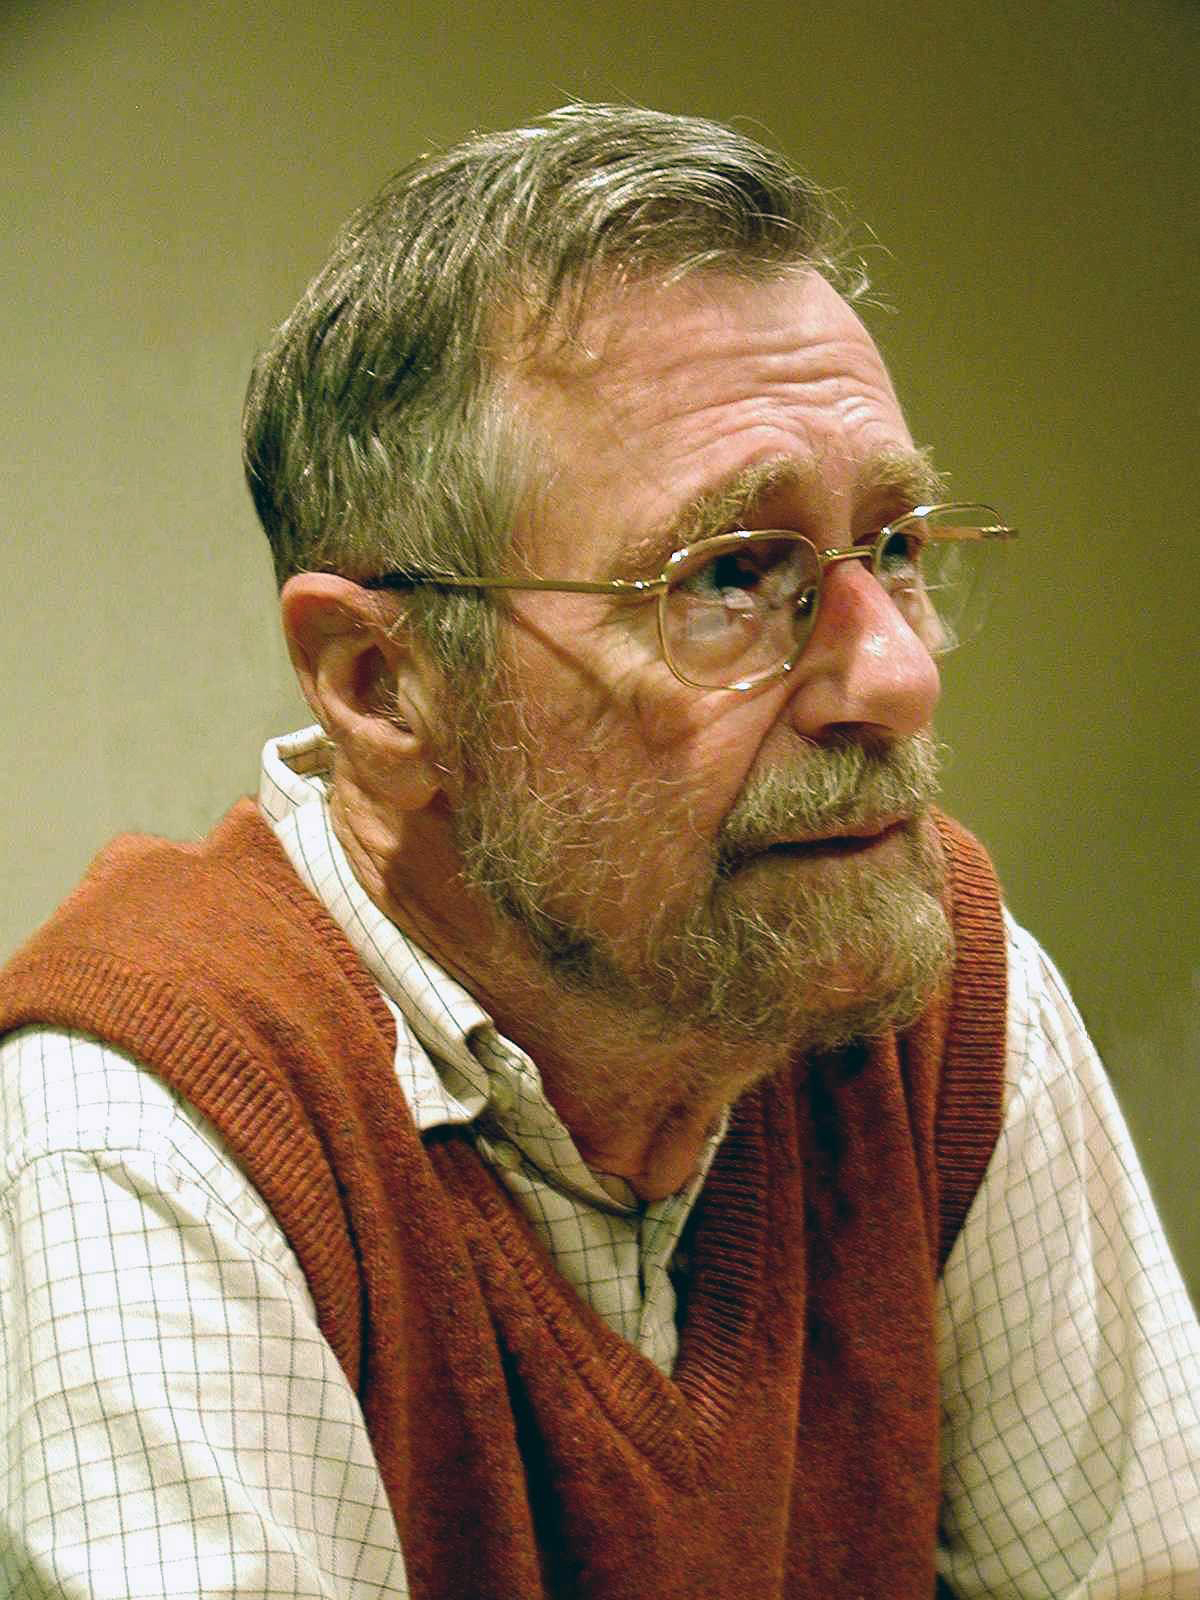
\includegraphics[height=4.5cm]{graph/dijkstra}
                \caption*{Quelle: \cite{wiki:dijkstra}}
            \end{figure}
        \end{minipage}
        \hfill
        \begin{minipage}{0.55\textwidth}
            \textit{„Program testing can be used to show the presence of bugs, but never to show their absence!.“} \\\\Edsger W. Dijkstra
        \end{minipage}
\end{frame}

\outlineSubframe{Komplexitätsanalyse}

\begin{frame}{Speicherkomplexität}{Wie lässt sich diese messen?}
    \begin{itemize}[<+->]
        \item Wie schon erwähnt: Der verbrauchte Speicher ist Sprach- und Rechnerabhängig
        \item Mögliche Lösung über Definition von Referenzsprache und -system
        \item Messungen sind allerdings nicht repräsentativ
        \item Deswegen wird in der formalen Informatik mit dem \textit{Random-Access-Machine}(RAM) Modell gearbeiteet
        \begin{itemize}
            \item Besteht im Grunde ausabzählbar unendlich vielen addressierbaren Speicherzellen
            \item Für einen Algorithmus wird dann bestimmt, wie viele Speicherzellen genutzt werden müssen
            \item Dies entspricht dann der Speicherkomplexität
        \end{itemize}
    \end{itemize}
\end{frame}

\begin{frame}{Laufzeitkomplexität}{Grundlegendes}
    \begin{itemize}[<+->]
        \item Gleiches Problem wie bei der Speicherkomplexität
        \item Deswegen hier ähnliches Modell:
        \begin{itemize}
            \item Man bestimmt die Anzahl von "`atomaren Operationen"' des Algorithmus
            \item Diese Operationen sind vergleichbar mit Assembler-Befehlsrepertoire
        \end{itemize}
        \item Beispiele für atomare Operationen:
        \begin{itemize}
            \item Addition/Subtraktion/Multiplikation/Division zweier Zahlen
            \item Lesen einer Variable von einer Speicheradresse
            \item Schreiben einer Variable an eine bestimmte Adresse
            \item Random Access in Arrays
            \item Vergleich zweier Zahlen
        \end{itemize}
        \item Angabe benötigten Operationen über $\tau(N)=x$
    \end{itemize}
\end{frame}

\begin{frame}[fragile]{Beispiel einer Komplexitätsanalyse}{Vertauschen zweier Zahlen I}
\lstset{style=java}
\begin{onlyenv}<1>
\begin{lstlisting}
public void swap(int first, int second){
    int tmp = first;
    first = second;
    second = tmp;
}
\end{lstlisting}
\end{onlyenv}

\begin{onlyenv}<2-|handout:0>
\begin{lstlisting}
public void swap(int first, int second){
    int tmp = first;    //1 Operation
    first = second;     //1 Operation
    second = tmp;       //1 Operation
}
\end{lstlisting}
\end{onlyenv}

\begin{itemize}
    \item Laufzeitkomplexität: \visible<3-|handout:0>{$\tau(N)=3$}
    \item<4-> Speicherkomplexität(In Byte): \visible<5-|handout:0>{$\tau(N)=12$}
\end{itemize}
\end{frame}

\begin{frame}[fragile]{Beispiel einer Komplexitätsanalyse}{Vertauschen zweier Zahlen II}
\lstset{style=java}
\begin{onlyenv}<1>
\begin{lstlisting}
public void swap(int first, int second){
    first = first + second;
    second = first - second;
    first = first - second;
}
\end{lstlisting}
\end{onlyenv}
\begin{onlyenv}<2-|handout:0>
\begin{lstlisting}
public void swap(int first, int second){
    first = first + second;     //2 Operationen
    second = first - second;    //2 Operationen
    first = first - second;     //2 Operationen
}
\end{lstlisting}
\end{onlyenv}


\begin{itemize}
    \item Laufzeitkomplexität: \visible<3-|handout:0>{$\tau(N)=6$}
    \item<4-> Speicherkomplexität(In Byte): \visible<5-|handout:0>{$\tau(N)=8$}
\end{itemize}
\end{frame}

\begin{frame}{Probleme und Probleminstanzen}
    \begin{itemize}[<+->]
        \item Komplexität ist selten statisch
        \item In der Regel von Problem und der konkreten \textit{Probleminstanz} abhängig
        \begin{itemize}
            \item Problem: z.B. Das Sortieren einer Liste
            \item Probleminstanz: konkrete Liste die sortiert werden soll, z.B. $(7, 3, 12, -5, 45)$
        \end{itemize}
        \item Die Probleminstanz hat meist einen oder mehrere dynamische Faktoren von denen die entgültige Komplexität abhängt
        \begin{itemize}
            \item Für Sortieren: \visible<+-|handout:0>{Länge der Liste}
        \end{itemize}
        \item Angegeben werden in der Komplexität nur noch die skalierenden Faktoren: $O(N)$
    \end{itemize}
    
    Vgl. \cite{ottmann2017} S. 3 ff
\end{frame}

\begin{frame}[fragile]{Dynamische Komplexität}{Ein Beispiel}
\lstset{style=java}
\begin{onlyenv}<+>
\begin{lstlisting}
//A-> Array mit Elementen, n->Länge von A
int sumList(int[] A, int n){
    int sum = 0;
    for(int i=0;i<n;i++){
        sum+=A[i]
    }
    return sum;
}
\end{lstlisting}
\end{onlyenv}

\begin{onlyenv}<+-|handout:0>
\begin{lstlisting}
//A-> Array mit Elementen, n->Länge von A
int sumList(int[] A, int n){
    int sum = 0;            //Kosten: 1, Anzahl: 1 mal
    for(int i=0;i<n;i++){   //Kosten: 2, Anzahl: n+1 mal
        sum+=A[i]           //Kosten: 3, Anzahl: n mal
    }
    return sum;             //Kosten: 1, Anzahl: 1 mal
}
\end{lstlisting}
\end{onlyenv}


\visible<+-|handout:0>{$ \tau(n) = 1 + 2\cdot(n+1) +  3n + 1 $}

\visible<+-|handout:0>{$ \tau(n) = 1+ 2n + 2 + 3n +1 $}

\visible<+-|handout:0>{$ \tau(n) = 4n + 4 $}
\visible<+-|handout:0>{$ \tau(n) = c_1n+c_2 $}

\visible<+-|handout:0>{$\Rightarrow O(n)$}
\end{frame}

\begin{frame}{Unterschiedliche Laufzeiten von Algorithmen}
    \begin{itemize}[<+->]
        \item Bisher betrachtete Algorithmen hatten (für gegebenes $N$) feste Komplexität
        \item Algorithmen können jedoch für gleiches $N$ verschiedene Laufzeiten haben
        \begin{itemize}
            \item Warum?
            \item<handout:0> Zum Beispiel bei Verzweigung innerhalb des Algorithmus (z.B. durch gesonderte Betrachtung besonderer Listenelemente o.Ä.)
        \end{itemize}
        \item Beispiel: Leicht angepasste Variante unseres Algorithmus zum addieren von geraden Zahlen:
    \end{itemize}
\end{frame}

\begin{frame}[fragile]{Addieren aller geraden Zahlen einer Liste}
\lstset{style=java}
\begin{onlyenv}<1>
\begin{lstlisting}
public int calculate(int[] data, int n){
    int res = 0;
    for(int i=0;i<n;i++){
        if(data[i]%2 == 1){
            res+=data[i];
        }else{
            res += data[i]*data[i];
        }
    }
    return res;
}
\end{lstlisting}
\end{onlyenv}
\begin{onlyenv}<2|handout:0>
\begin{lstlisting}
public int calculate(int[] data, int n){
    int res = 0;            //Kosten: 1, 1 mal
    for(int i=0;i<n;i++){   //Kosten: 2, (n+1) mal
        if(data[i]%2 == 1){ //Kosten: 3, n mal
            res+=data[i];   //Kosten: 3, ? mal
        }else{
            //Kosten: 5, ? mal
            res += data[i]*data[i];
        }
    }
    return res;
}
\end{lstlisting}
\end{onlyenv}
\end{frame}

\begin{frame}{Best- und Worst-Case Execution Time}
    \begin{itemize}[<+->]
        \item Für diese Fälle gibt es prinzipiell drei Betrachtungsweisen
        \begin{itemize}
            \item Best-Case Execution Time
            \item Worst-Case Execution Time
            \item Average Execution Time
            \item Frage: Welche ist für die Komplexitätsbetrachtung relevant?
        \end{itemize}
        \item Average Execution Time lässt sich nur schwer bestimmen
        \begin{itemize}
            \item Reiner Durchschnitt aus Best- und Worst-Case nicht praktikabel
            \item Beschaffenheit der Probleminstanzen und deren Verteilung müsste bekannt sein
            \item Ist jedoch selten der Fall
        \end{itemize}
    \end{itemize}
\end{frame}

\begin{frame}{Best- und Worst-Case Execution Time}
    \begin{itemize}
        \item In der Regel ist die Worst-Case Execution Time relevant
        \begin{itemize}
            \item Simpel zu bestimmen
            \item Dadurch kann sichergestellte werden, dass der Algorithmus \textbf{maximal} die angegebene Zeit benötigt
            \item insbesondere relevant für Echtzeitsysteme
        \end{itemize}
    \end{itemize}
Vgl. \cite{ottmann2017} S. 3ff
\end{frame}

\begin{frame}{Gängige Komplexitätsfaktoren}{Vgl. \cite{ottmann2017}}
    \begin{itemize}[<+->]
        \item In der Regel begegnet man den folgenden Komplexitäten bei der Analyse(In Abhängigkeit von $N$):
        \begin{itemize}
            \item Kein Wachstum: $O(1)$
            \item Logarithmisches Wachstum: $O(\log N)$
            \item Lineares Wachstum: $O(N)$
            \item $N$-log $N$-Wachstum: $O(N\cdot\log N)$
            \item Polynomiales Wachstum: $O(N^2)$, $O(N^3)$...
            \item Exponentielles Wachstum: $O(2^N)$, $O(3^N)$...
            \item Faktorielles Wachstum: $O(N!)$
        \end{itemize}
        \item Praktikabel sind maximal Algortihmen mit polynomialen Wachstum
        \item Exponentielle und faktorielle Algorithmen wachsen zu schnell an
    \end{itemize}
\end{frame}

\begin{frame}{Komplexität von Algorithmen}{Visueller Vergleich}
\begin{figure}
\centering
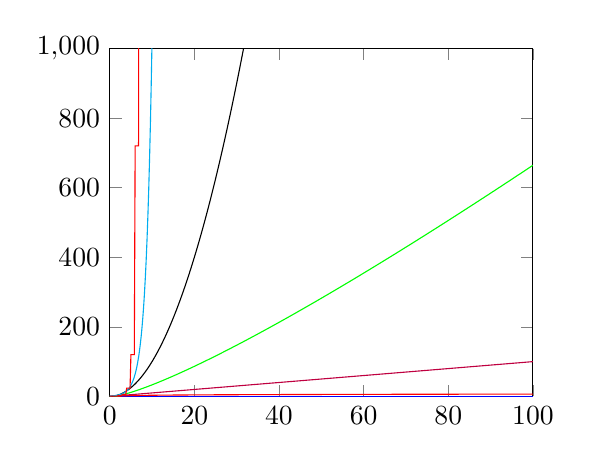
\begin{tikzpicture}
\begin{axis}[height=6cm,ymin=0,xmin=0,xmax=100,ymax=1000,domain=0:100,restrict x to domain*=0:100, restrict y to domain*=0:2500,samples=500]
  \addplot[blue]{1};
  \addplot[red]{log2(x)};
  \addplot[purple]{x};
  \addplot[green]{x*log2(x)};
  \addplot[black]{x^2};
  \addplot[cyan]{2^x};
  \addplot[red]{x!};
\end{axis}
\end{tikzpicture}
\end{figure}
\end{frame}

\begin{frame}[fragile]{Beispiele für Komplexität}{Kein Wachstum $O(1)$}
\lstset{style=java}
\begin{lstlisting}
public void swap(int[] data, int first, int second){
    int tmp = data[first];
    data[first] = data[second];
    data[second] = tmp;
}
\end{lstlisting}
\begin{itemize}
    \item Algorithmus ist in keiner Weise von der Länge von \texttt{data} abhängig (Abgesehen von eventueller Fehlerbetrachtung)
\end{itemize}
\end{frame}

\begin{frame}[fragile]{Beispiele für Komplexität}{Logarithmisches Wachstum $O(\log N)$}
\lstset{style=java}
\begin{lstlisting}
public void logNComplexity(int n){
    for(int i=1; i<=n; i = i * 2){
        System.out.println(i);
    }
}
\end{lstlisting}
\begin{itemize}
    \item Indikator für Logarithmisches Wachstum:
    \begin{itemize}
        \item Zählvariable steigt multiplikativ/verringert sich durch Division
        \item Größe der Probleminstanz verringert sich in jedem Schritt mit bestimmtem Faktor
    \end{itemize}
    \item Basis des Logarithmus ist nicht von Relevanz, da nur konstanter Faktor
    \item In der Regel handelt es sich aber um $\log_2$
    \item Beispiel: Binäre Suche
\end{itemize}
\end{frame}

\begin{frame}[fragile]{Beispiele für Komplexität}{Lineares Wachstum $O(N)$}
\lstset{style=java}
\begin{lstlisting}
public int sum(int[] data, int n){
    int res=0;
    for(int i=0;i<n;i++){
        res+=data[i];
    }
    return res;
}
\end{lstlisting}
\begin{itemize}
    \item Grundlegend alle Schleifen, die von 0 bis $N$ iterieren (Mit Schrittweite 1)
    \item Beispiele:
    \begin{itemize}
        \item Summen von Listen
        \item Finden von Mini-/Maxima in unsortierten Listen
    \end{itemize}
\end{itemize}
\end{frame}

\begin{frame}[fragile]{Beispiele für Komplexität}{$N$-log $N$-Wachstum $O(N\cdot \log N)$}
\lstset{style=java}
\begin{lstlisting}
public void nlogNComplexity(int n){
    for(int i=0;i<n;i++){
        for(int j=0;j<n;j=j*2){
            System.out.println(i);
            System.out.println(j);
        }
    }
}
\end{lstlisting}
\begin{itemize}
    \item Entsteht durch die Kombination von linearem und logarithmischen Wachstums
    \item Beispiele:
    \begin{itemize}
        \item Heap Sort
        \item Quick Sort
    \end{itemize}
\end{itemize}
\end{frame}

\begin{frame}[fragile]{Beispiele für Komplexität}{Polynomiales Wachstum $O(N^x)$}
\lstset{style=java}
\begin{lstlisting}
//Unter der Annahme, dass data ein n*n Array ist
public void print2DArray(int[][] data, int n){
    for(int i=0;i<n;i++){
        for(int j=0;j<n;j++){
            System.out.println(data[i][j]);
        }
    }
}
\end{lstlisting}
\begin{itemize}
    \item Entsteht durch die Verschachtelung mehrerer $O(N)$ Algorithmen
    \item Beispiele:
    \begin{itemize}
        \item Insertion Sort
        \item Traversieren von N-Dimensionalen Arrays
    \end{itemize}
\end{itemize}
\end{frame}

\begin{frame}{Beispiele für Komplexität}{Exponentielles Wachstum $O(x^N)$}
\begin{itemize}
    \item Hier ist mir leider kein leichtes Codebeispiel eingefallen
    \item Beispiele:
    \begin{itemize}
        \item Bruteforce von Passwörtern 
        \item Damenproblem (mit naiver Implementierung)
    \end{itemize}
\end{itemize}
\end{frame}

\begin{frame}[fragile]{Beispiele für Komplexität}{Faktorielles Wachstum $O(N!)$}
\lstset{style=java}
\begin{lstlisting}
public void factorial(int n){
    for(int i=0;i<n;i++){
        System.out.println(i);
        factorial(n-1);
    }
}
\end{lstlisting}
\begin{itemize}
    \item Häufig in rekursiven Algorithmen
    \item Beispiele:
    \begin{itemize}
        \item Finden aller Permutationen in einem Array
        \item Travelling Salesman Problem (Primitiver Ansatz)
    \end{itemize}
\end{itemize}
\end{frame}